\subsection{Results}
To compare the two localization methods, a UMB-mark test was conducted, as described earlier.

%The UMB-test was conducted as follows:
%
%\begin{enumerate}
%\item The robots start position of the robots wheels where marked on the floor.
%\item The robot then drives 1m forward, using the given library, and then holds a break. If it returned to this point for the 20th time, it stops. \label{item:driveForward}
%\item During the robots pause, the position of the robots wheels were, again, marked on the floor.
%\item The robot then turns $90^{\circ}$ to the left and continues then from point \ref{item:driveForward}. 
%\end{enumerate}

During the course of this test data from the encoders and 2D laser scanner were collected for off-line processing. 
Furthermore the actual position of the robot was measured.
%Afterwards the start, end and intermediate positions of the robot were measured.

The data was then used to find the robots position given the two datasets. 
Because of faults first discovered later, there were inconsistencies in the data collection.
The datasets where hence reduced to include only the beginning of the dataset till just before the point where the corruption was too great to be used for positioning the robot on the map.

The positions calculated are seen in figure \ref{fig:comparisonOfEncoderVSScanner}. 


\begin{figure}[H]
\centering
\makebox[\textwidth][c]{
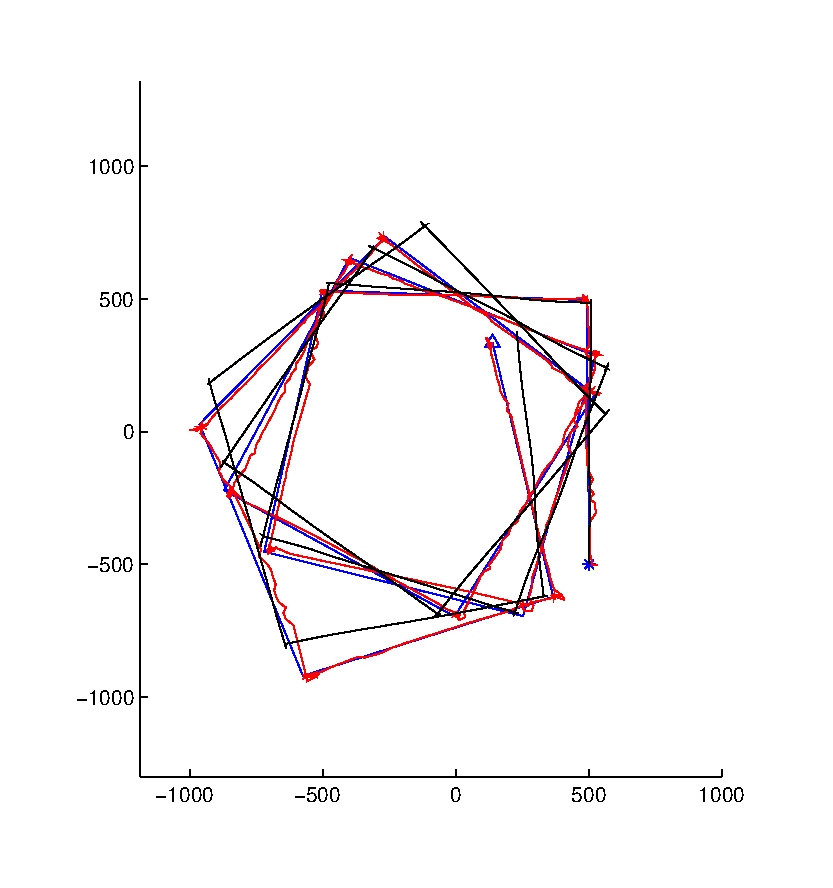
\includegraphics[width = 15cm,trim= 1cm 1cm 1cm 1cm ,clip=true]{graphics/comparison_encoderVSscanner}}
\caption[Comparison of the two localization methods.]{Comparison of the two localization methods. The blue line is the actual path travelled, $*$ is start and $\Delta$ is end position. The red line is the 2D laser scanner and the black line the encoder data.}
\label{fig:comparisonOfEncoderVSScanner}
\end{figure}

It can be seen that the 2D laser scanner predicts a position of the robot that is deviating from the ideal line between the two points where the robot moves.
This can partially be some small error in the lines found in the datasets, but also because the robot itself, moved a bit sinusoidal during the data collection.

The deviation of the two models for calculating the position of the robot is seen in figure \ref{fig:deviationOfEncoderVSScanner}.
The figure shows the deviation of the robot at the positions where it paused. 
This is because they are the only points, for the actual robot position, that were measured in the course of the data collection.

\begin{figure}[H]
\centering
\includegraphics[width = 13cm]{graphics/deviation_encoderVSscanner}
\caption[Deviation of the two localization methods.]{Deviation of the two localization methods. The red line is the 2D laser scanner and the black line the encoder data.}
\label{fig:deviationOfEncoderVSScanner}
\end{figure}

From figure \ref{fig:deviationOfEncoderVSScanner} it can be seen that the error accumulates over time when using the encoders to measure the position. The data from the 2D laser scanner, however, predicts its position considerably better with a much more steady deviation.
It can hence be concluded that the 2D laser scanner is considerably better than the encoder in the long run. The encoders can, however, still be used to accurately decide the robots position when travelling short distances in case the scanner fails.